\paragraph{В четвертой} главе приводится полунатурный эксперимент по проверке рабочих характеристик алгоритма
оценки частоты широкополосного сигнала на фоне аддитивного белого гауссового шума и интерференционной помехи.
В качестве аппаратной платформы использовалась плата разработанная мной в процессе дипломного проектирования.
В качестве микросхемы захвата сигнала использовался чип от компании Maxim Semiconductor - MAX2769.

{\bf{добавить графики полунатурного моделирования}}






%\paragraph{В четвертой} главе приводится имитационное моделирование развиваемых алгоритмов. В качестве алгоритма
%для сравнения используется параллельный коррелятор с алгоритмом уточнения частоты.
%
%\noindent{\begin{figure}[H]
%\center\scalebox{0.65}{\includegraphics[width=1\linewidth]{modeling_general.eps}}
%	\caption{Схема эксперимента}
%	%\label{pic:ar_dma_probability}
%\end{figure}}
%
%\underline{Алгоритм} оценки параметров сигнала с расширенным спектром на фоне аддитивного белого шума.
%График вероятности оценки частоты в допустимом диапазоне входной расстройки представлен на рисунке
%\ref{pic:lpc_for_1_probability}. Моделирование проводилось с аддитивным шумом, заданным в полосе от 0 Гц до
%половины частоты дискретизации для одного, двух и трех шагов уточнения АКФ. В данном случае значение частоты дискретизации равно 16.368 МГц.
%\begin{figure}[H]
%\center\scalebox{1}{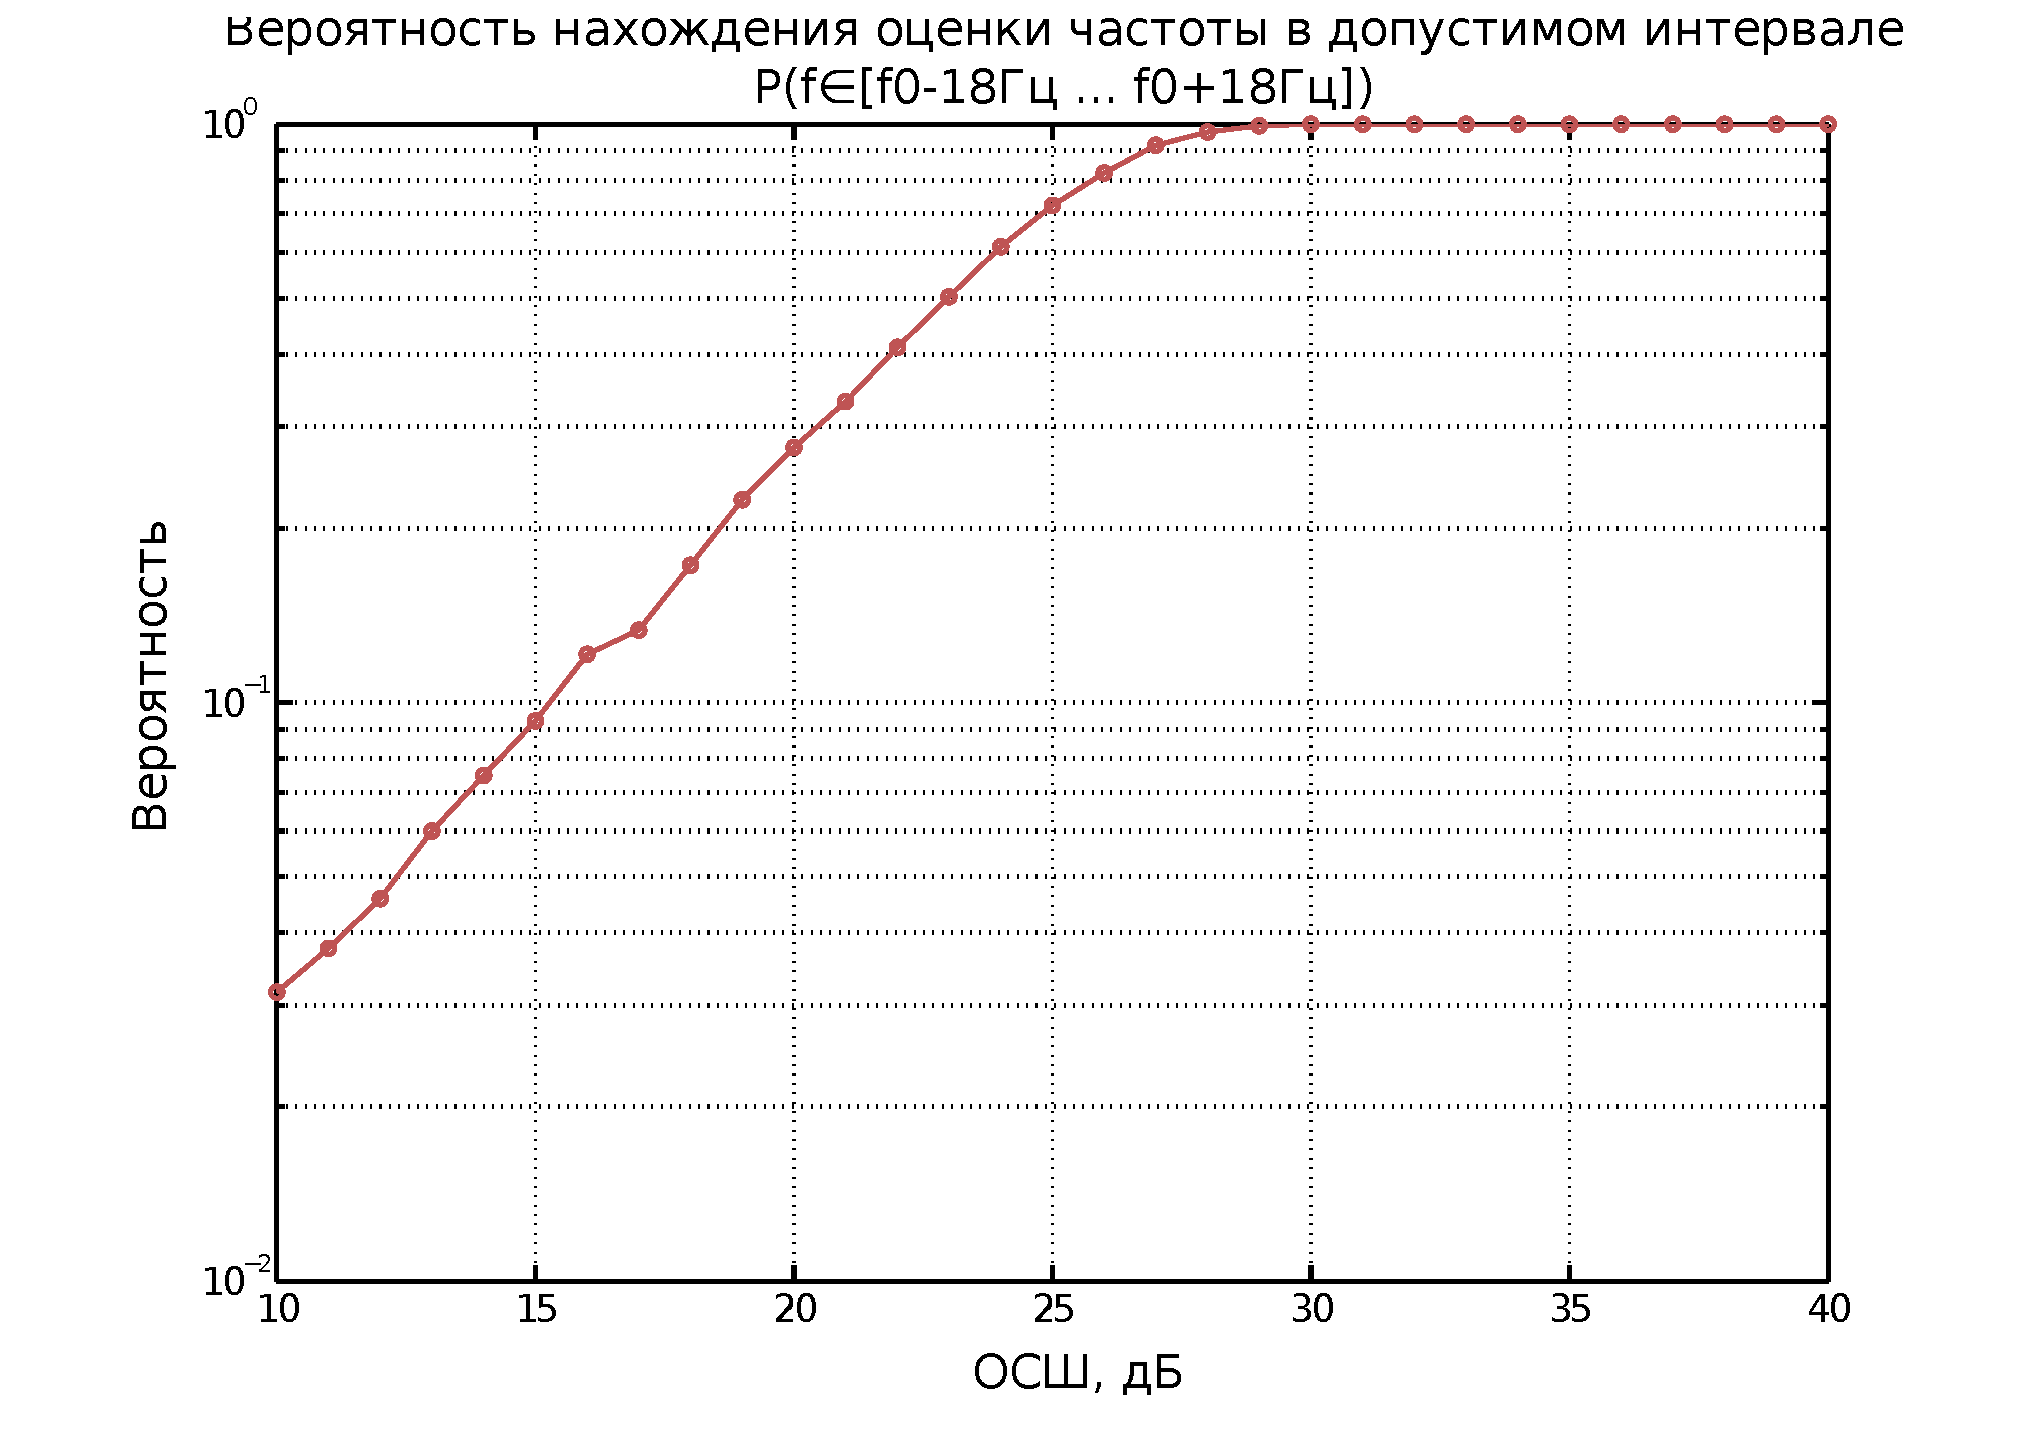
\includegraphics[width=1\linewidth]{lpc_for_1_probability.eps}}
%	\caption{Вероятность оценки частоты удовлетворяющей допустимой входной расстройке}
%	\label{pic:lpc_for_1_probability}
%\end{figure}
%
%Для оценки точности можно сравнить предлагаемый алгоритм с границей Крамера-Рао. Неравенство Крамера-Рао дает базу оценки, так
%как представляет минимальную дисперсию среди всех классов оценщиков.
%\begin{figure}[H]
%\center\scalebox{1}{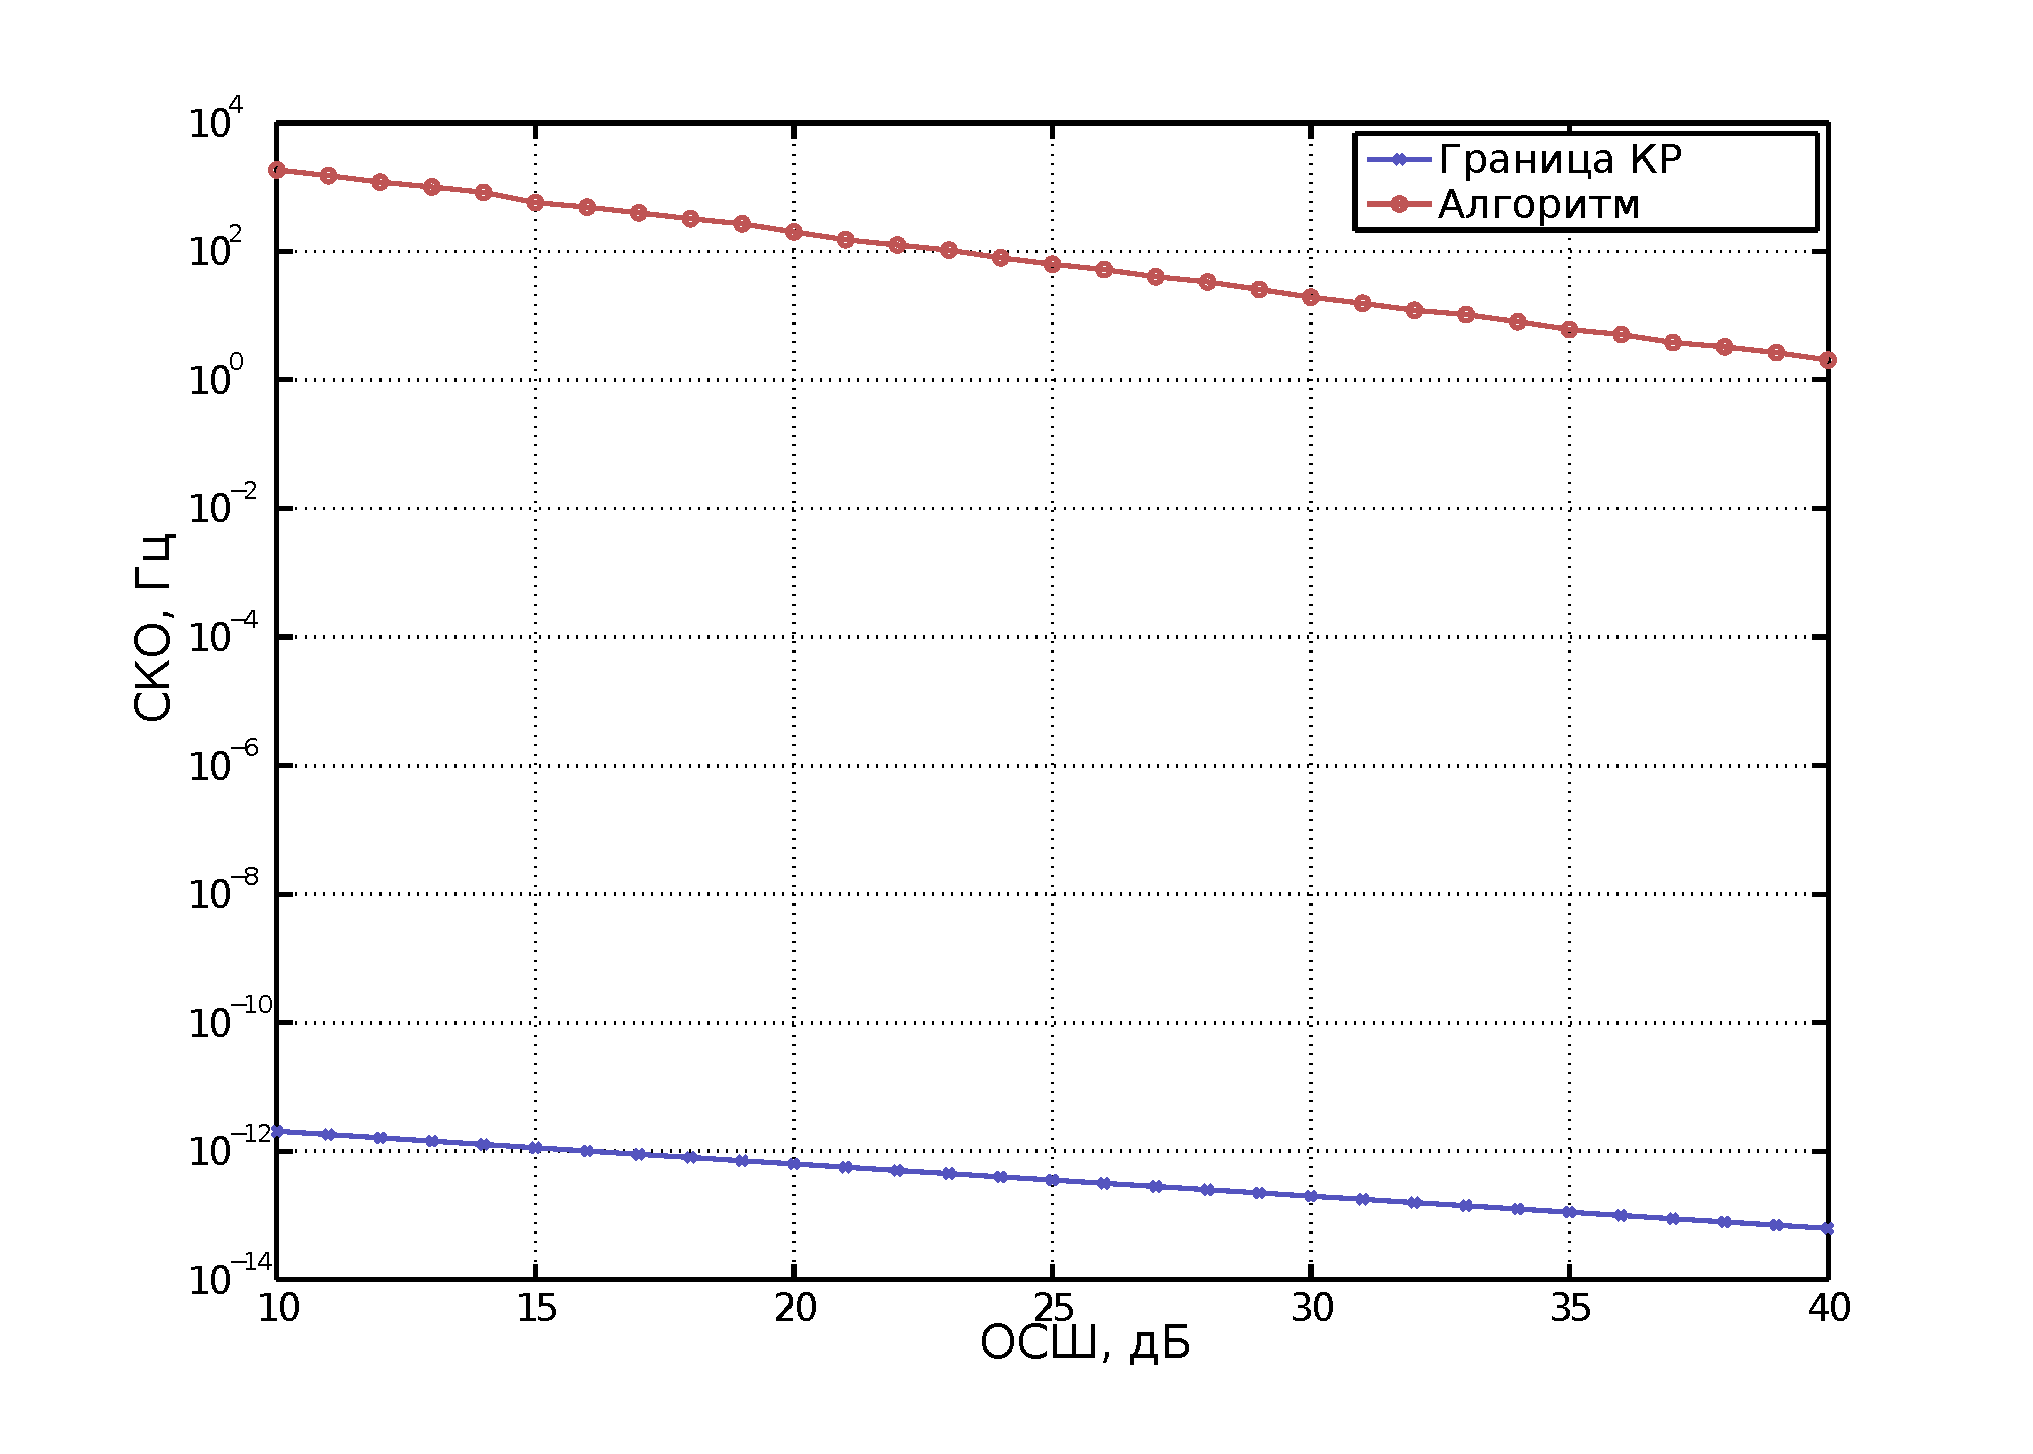
\includegraphics[width=1\linewidth]{crlb_vs_1sat_algo.eps}}
%	\caption{СКО ошибка оценки частоты и граница Крамера-Рао в задаче оценки частоты гармонического сигнала}
%	\label{pic:crlb_vs_1sat_algo}
%\end{figure}
%
%%%%%%%%%%
%\underline{Алгоритм} оценки параметров ШПС в условиях интерференции и аддитивного белого шума
%(Delay and Multiply Approach + уточненный АР).
%
%График вероятности оценки частоты в допустимом диапазоне входной расстройки представлен на рисунке
%\ref{pic:ar_dma_probability}. Моделирование проводилось с аддитивным шумом, заданным в полосе от 0 Гц до
%половины частоты дискретизации для одного, двух и трех шагов уточнения АКФ. В данной имитационной модели значение частоты дискретизации равно 16.368 МГц.
%\begin{figure}[H]
%\center\scalebox{1}{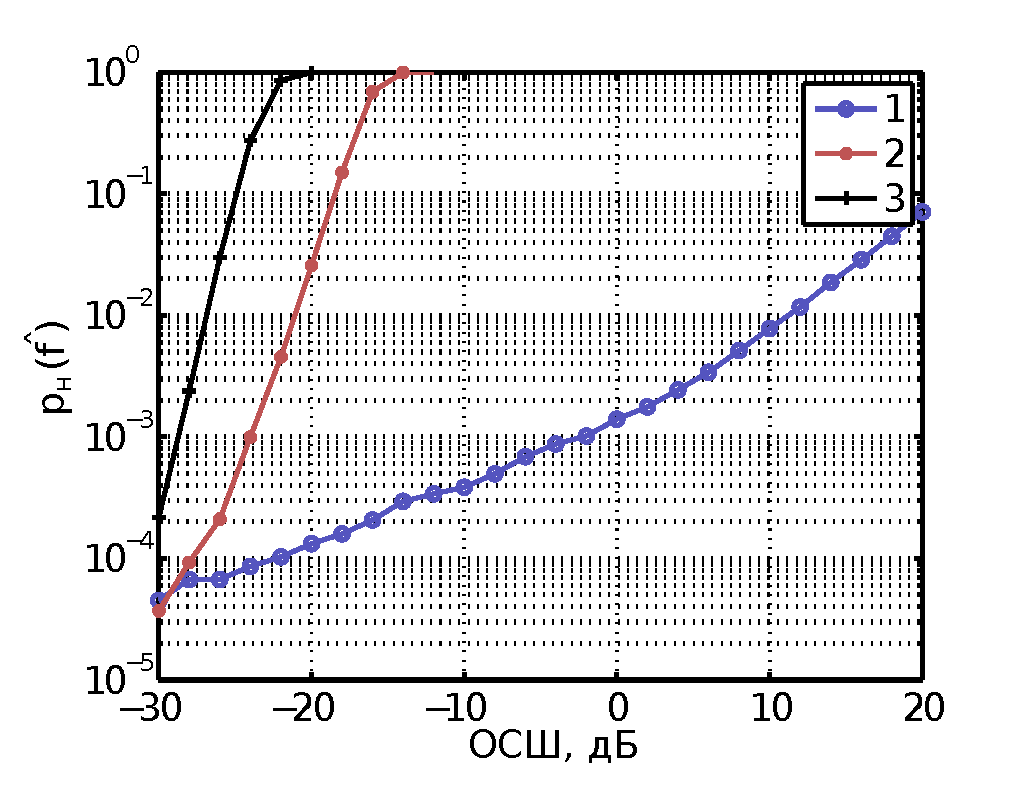
\includegraphics[width=1\linewidth]{ar_dma_probability.eps}}
%	\caption{Вероятность оценки частоты удовлетворяющей допустимой входной расстройке}
%	\label{pic:ar_dma_probability}
%\end{figure}
%
%Так же интересным является сравнение качество оценки частоты. График СКО ошибки при оценке частоты в зависимости
%от ОСШ представлен на рисунке \ref{pic:crlb_vs_snr}. Для сравнения так же взята граница Крамера-Рао (КР).
%\begin{figure}[H]
%\center\scalebox{1}{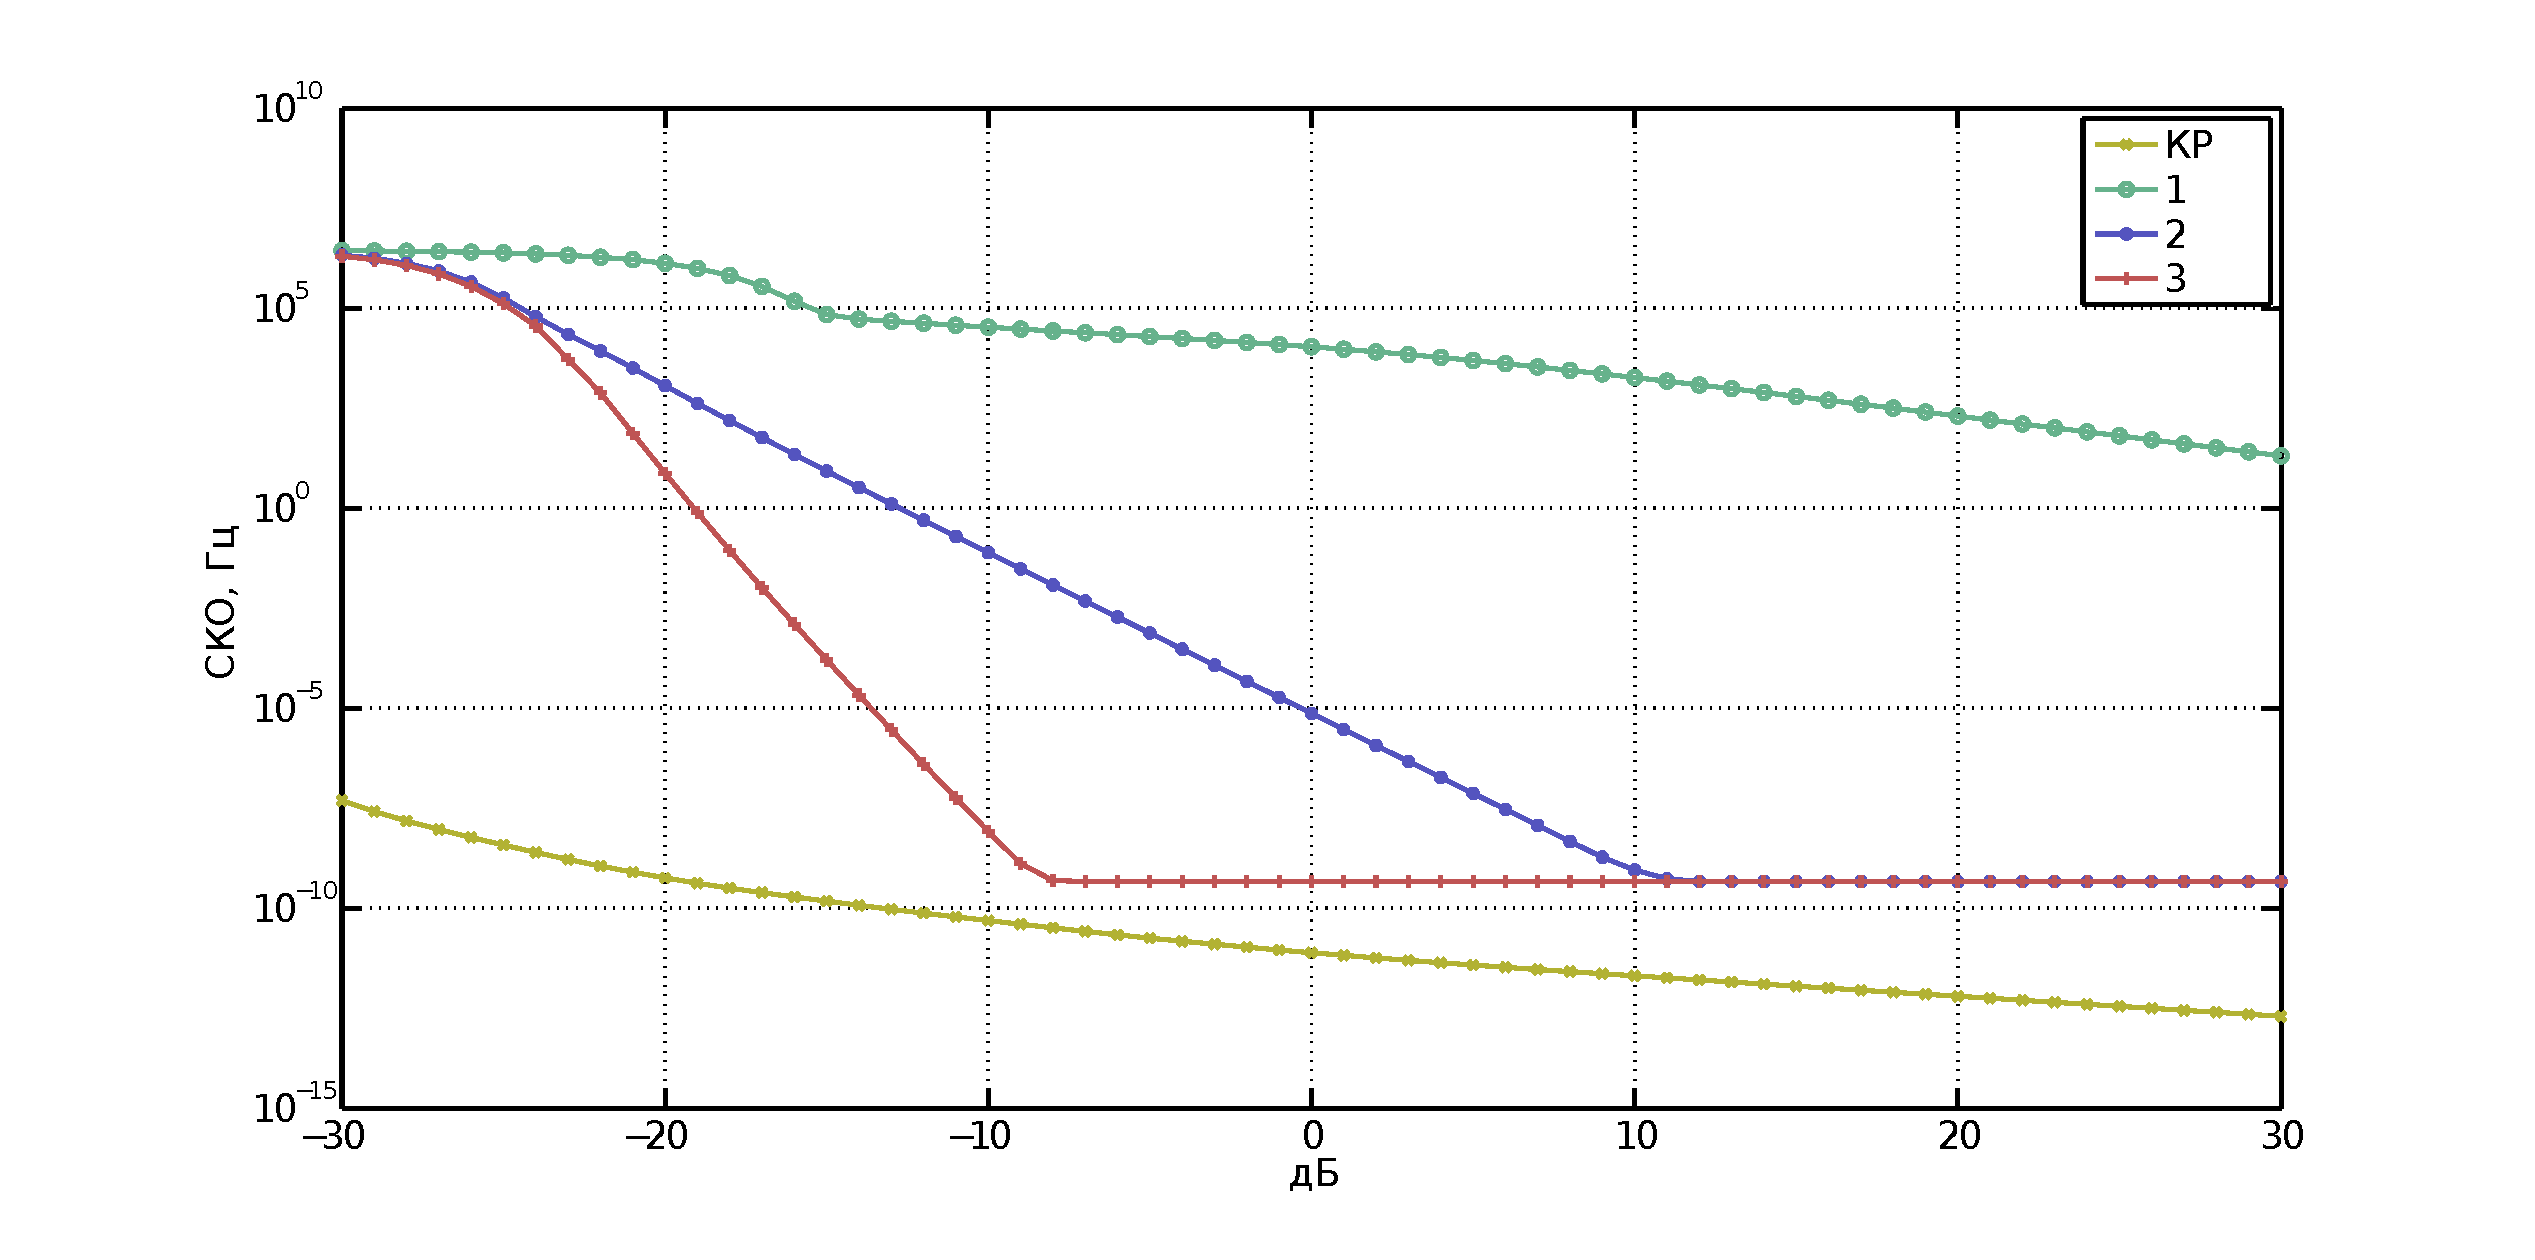
\includegraphics[width=1\linewidth]{crlb_vs_snr.eps}}
%	\caption{СКО ошибка оценки частоты и граница Крамера-Рао в задаче оценки частоты гармонического сигнала}
%	\label{pic:crlb_vs_snr}
%\end{figure}
